\chapter{Interaction Diagram of OMPD Components}
\index{ompd diagram}
\label{chap:ompd_diagram}


   \begin{figure}[h]
    \centering
        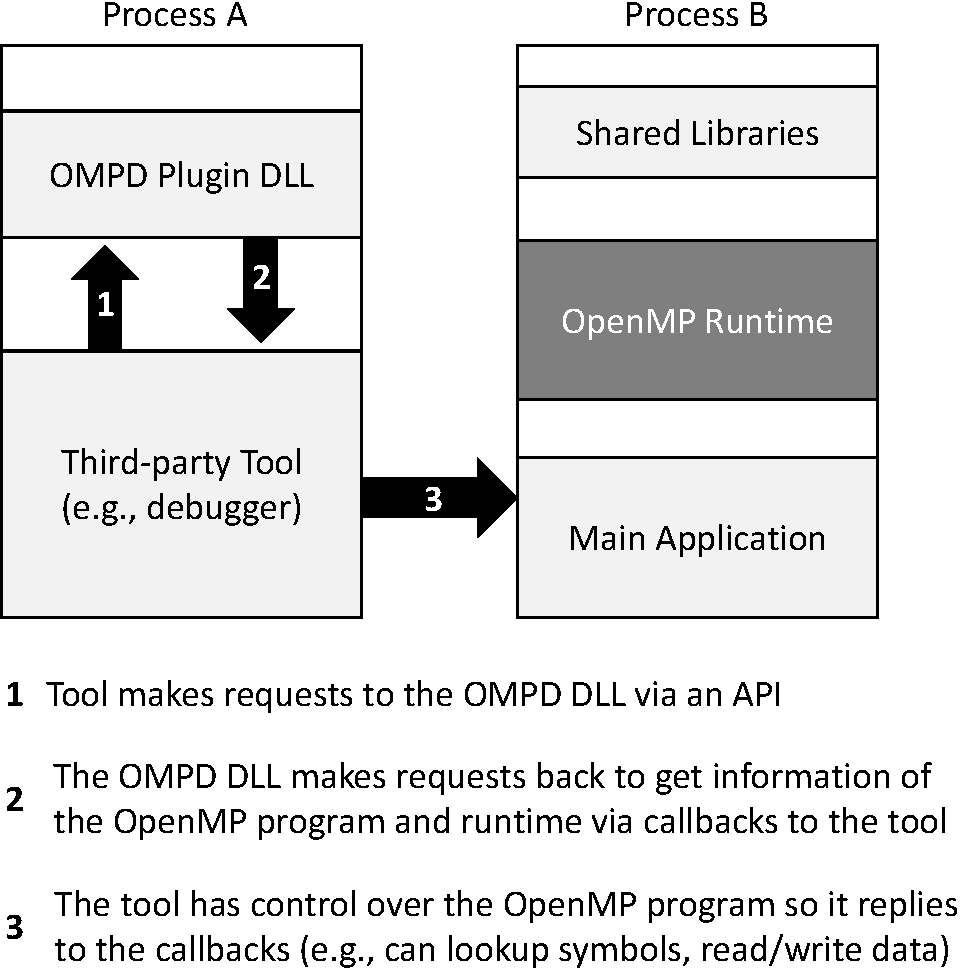
\includegraphics[width=3.5in]{appendices/ompd_diagram.pdf}
    \caption{Interaction Diagram of OMPD Components}
    \label{fig:ompd_diagram}
\end{figure}

The figure shows how the different components of OMPD fit together. The \emph{third-party tool} loads
the OMPD library
that matches the OpenMP runtime being used by the OpenMP program. The
library exports the API defined in
\specref{sec:ompd-overview}, which the tool uses to get
OpenMP information about the
OpenMP program. The OMPD
library will need to look up the symbols, or read data out of the
OpenMP program. It does not do this directly,
but instead asks the tool to perform these operations
for it using a callback interface exported
by the tool.

This architectural layout insulates the tool from the details of the
internal structure of the
OpenMP runtime. Similarly, the OMPD library does not need to be
concerned about how to access
the OpenMP program. Decoupling the library and tool in this
way allows for flexibility in how the OpenMP program and tool are deployed, so that, for example,
there is no requirement that tool and OpenMP program
execute on the same machine.

\begin{crossrefs}
\item OMPD interface, see \specref{sec:ompd-overview}.
\end{crossrefs}

